
-	Roofline model \\
-	Identifying functions that are memory intensive \\

\subsection{Jacobi}
The main function in Jacobi is the $stencil\_jacobi$ function which is a memory bound kernel (see Fig.~\ref{fig:roof-jacobi}). 

\begin{figure}[h]%[bp]
\begin{center}
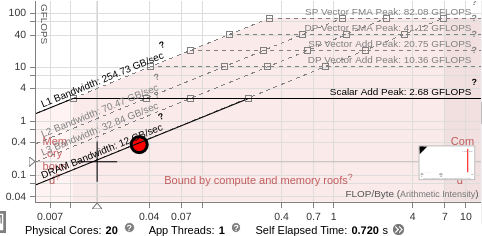
\includegraphics[width=1\linewidth]{MEMSYS22/figures/roofline/jacobi.png}
\end{center}
  \vspace{-0.1in}
\caption{Positioning of Jacobi kernel in Roofline}
\label{fig:roof-jacobi}
\vspace{-0.2in}
\end{figure}

\subsection{MiniAMR}
The main computation function in miniAMR is the $stencil\_calc$  which is a memory bound kernel (see Fig.~\ref{fig:roof-miniamr}). 

\begin{figure}[h]%[bp]
\begin{center}
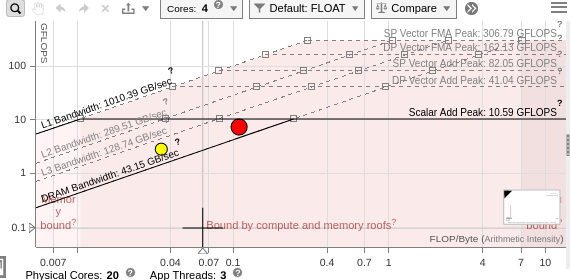
\includegraphics[width=1\linewidth]{MEMSYS22/figures/roofline/miniamr.png}
\end{center}
  \vspace{-0.1in}
\caption{Positioning of the main compute kernel of MiniAMR app in Roofline. Here the red circle indicates the $stencil\_calc$ function }
\label{fig:roof-miniamr}
\vspace{-0.2in}
\end{figure}

\subsection{SimpleMOC}
The main computation function in SimpleMOC is the $attenuate\_fluxes$  which is a memory bound kernel (see Fig.~\ref{fig:roof-simplemoc}). 

\begin{figure}[h]%[bp]
\begin{center}
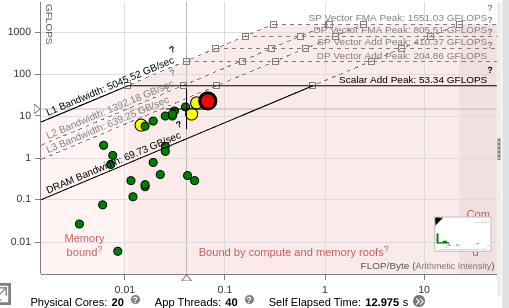
\includegraphics[width=1\linewidth]{MEMSYS22/figures/roofline/simplesoc.png}
\end{center}
  \vspace{-0.1in}
\caption{Positioning of the main compute kernel of MiniAMR app in Roofline. Here the red circle indicates the $attenuate\_fluxes$ function }
\label{fig:roof-simplemoc}
\vspace{-0.2in}
\end{figure}


%\begin{figure}[t!]
%\centering
%\includegraphics[width=70mm, height= 50mm]{figure/pmtj.pdf}
%%\vspace{.5em} 
%\caption{STT-MRAM cell}
%%\vspace{-1.5em} 
%\label{fig:pmtj}
%%\vspace{-0.3cm}   
%\end{figure} 
%
%
%
%
%  
%\looseness -1
%
%
%
%\begin{figure}[t!]
%\centering
%\includegraphics[width=\columnwidth]{figure/DeviceCapacity.pdf}
%%\vspace{.5em} 
%\caption{DRAM and STT-MRAM capacity growth in years} %\pr{23-Feb: Kazi, do we have any data from after 2016? Take care of this only if you have some extra time. }}
%%\vspace{-1.5em} 
%\label{fig:Capa}
%\vspace{-0.3cm}  
%\end{figure}  


%
%
%\begin{table}[t!]
%%\normalsize
%\small
%\caption{\mbox{DRAM vs STT-MRAM for embedded real-time systems}}
%\centering
%%    \begin{tabularx}{\columnwidth}{lcc}
%    \begin{tabularx}{7.2cm}{lcc}
%\toprule
%    % \hline
%    Feature & DRAM & STT-MRAM \\
%\midrule
%Radiation-hard & - & +++ \\
%Standby power  & - & +++ \\
%Temperature tolerance & + & +++ \\
%Storage capacity & ++ & ++ \\
%Access speed   & +++ & ++ \\
%Endurance      & ++ & +++ \\
%\bottomrule
%   \end{tabularx}
%\label{table:compare}
%%\vspace{-0.5cm}
%\end{table}
%
%
%
%\begin{figure}[t!]
%\centering
%\includegraphics[width=\columnwidth]{figure/processor.png}
%\caption{Schematic view of the Next Generation Microprocessor~(NGMP)}
%\label{fig:processor}
%%\vspace{-0.4cm}
%\end{figure}









